% \begin{savequote}[75mm]
% This is some random quote to start off the chapter.
% \qauthor{Firstname lastname}
% \end{savequote}

\chapter{Hawkes Processes with Latent Network Structure}
\TODO{Rewrite the intro to focus on neurons, then cite other example areas}
Networks play a central role in modern data analysis, enabling us to reason about systems by studying the relationships between their parts.  Most often in network analysis, the edges are given.  However, in many systems it is difficult or impossible to measure the network directly.  Examples of latent networks include economic interactions linking financial instruments and patterns of reciprocity in gang violence.  In these cases, we are limited to noisy observations of events associated with each node.  To enable analysis of these implicit networks, we develop a probabilistic model that combines mutually-exciting point processes with random graph models.  We show how the Poisson superposition principle enables an elegant auxiliary variable formulation and a fully-Bayesian, parallel inference algorithm.  We evaluate this new model empirically on several datasets.

\section{Introduction}
Many types of modern data are characterized via relationships on a network.  Social network analysis is the most commonly considered example, where the properties of individuals (vertices) can be inferred from ``friendship'' type connections (edges).  Such analyses are also critical to understanding regulatory biological pathways, trade relationships between nations, and propagation of disease.  The tasks associated with such data may be unsupervised (e.g., identifying low-dimensional representations of edges or vertices) or supervised (e.g., predicting unobserved links in the graph).  Traditionally, network analysis has focused on \emph{explicit network} problems in which the graph itself is considered to be the observed data.  That is, the vertices are considered known and the data are the entries in the associated adjacency matrix. A rich literature has arisen in recent years for applying statistical machine learning models to this type of problem, e.g., \citet{Liben-2007,Hoff-2008,Goldenberg-2010}.

In this paper we are concerned with \emph{implicit networks} that cannot be observed directly, but about which we wish to perform analysis.  In an implicit network, the vertices or edges of the graph may not be directly observed, but the graph structure may be inferred from noisy emissions.  These noisy observations are assumed to have been generated according to underlying dynamics that respect the latent network structure.

For example, trades on financial stock markets are executed thousands of times per second. Trades of one stock are likely to cause subsequent activity on stocks in related industries. How can we infer such interactions and disentangle them from market-wide fluctuations? Discovering latent structure underlying financial markets not only reveals interpretable patterns of interaction, but also provides insight into the stability of the market. In Section~\ref{sec:stability} we will analyze the stability of mutually-excitatory systems, and in Section~\ref{sec:financial} we will explore how stock similarity may be inferred from trading activity.

As another example, both the edges and vertices may be latent.  In Section~\ref{sec:chicago}, we examine patterns of violence in Chicago, which can often be attributed to social structures in the form of gangs.  We would expect that attacks from one gang onto another might induce cascades of violence, but the vertices (gang identity of both perpetrator and victim) are unobserved.  As with the financial data, it should be possible to exploit dynamics to infer these social structures.  In this case spatial information is available as well, which can help inform latent vertex identities.

In both of these examples, the noisy emissions have the form of events in time, or ``spikes,'' and our intuition is that a spike at a vertex will induce activity at adjacent vertices.  In this paper, we formalize this idea into a probabilistic model based on mutually-interacting point processes.  Specifically, we combine the Hawkes process \cite{Hawkes-1971} with recently developed exchangeable random graph priors.  This combination allows us to reason about latent networks in terms of the way that they regulate interaction in the Hawkes process.  Inference in the resulting model can be done with Markov chain Monte Carlo, and an elegant data augmentation scheme results in efficient parallelism. 

\section{Probabilistic Network Models}
\label{sec:graph_models}
Networks of~$N$ nodes can be represented by~${N\times N}$
matrices. Unweighted networks are binary adjacency matrices~$\bA$
where~${a_{m,n}=a_{m \to n}=1}$ indicates a directed edge from
node~$m$ to node~$n$. We use the arrow notation ($\to$) to remind the
reader of the directionality of the connection. When these edges have
weights associated with them, we can use a second matrix,~${\bW \in
  \reals^{N \times N}}$.  The complete network is then defined by the
elementwise product,~${\bA \odot \bW}$. The binary adjacency matrix
captures the sparsity pattern, and the real-valued wieght matrix
captures the strength of the connections. From a modeling perspective,
separating these two matrices allows us to separate our prior
intuitions about sparsity and strength. This is known as a
spike-and-slab model~\cite{Mitchell1988, Mohamed-2012}.


Arbitrarily complex models can be constructed by incorporating latent
variables into the prior distributions over~$\bA$ and~$\bW$.
Unsurprisingly, the same types of motifs that recur throughout
probabilistic modeling --- discrete mixture models and low-dimensional
factor models, for example --- also form the building blocks of
standard network models.  We briefly outline a few simple models that
are used in this and following chapters.


\begin{table}
\begin{center}
\begin{tabular}{c|c|c|c}
Name & $\boldeta$ & $\quad\theta_n\quad$ & $\rho_{m \to n}$ \\
\hline
Empty Model & --- &  --- & $0$ \\
Dense Model & --- & --- & $1$ \\
Bernoulli Model & $\rho$ & --- & $\rho$ \\
Stochastic Block Model & $\{\{\rho_{c \to c'}\}\}$ & $c_n$ & $\rho_{c_m \to c_n}$ \\
Latent Distance Model & $\gamma_0$ & $\bell_n$ & $\sigma(-||\ell_n - \ell_m||_2^2 + \gamma_0)$
\end{tabular}
\end{center}
\caption{Binary Adjacency Matrix Models}
\label{tab:A_models}
\end{table}

Table~\ref{tab:A_models} summarizes a few models for binary adjacency
matrices. In all cases, the distribution over~$\bA$ factorizes into a
product over edges,
\begin{align*}
  p(\bA \given \btheta, \boldeta)
  &= \prod_{m=1}^N \prod_{n=1}^N \distBernoulli(a_{m \to n} \given \theta_m, \theta_n, \boldeta) \\
  &= \prod_{m=1}^N \prod_{n=1}^N \distBernoulli(a_{m \to n} \given \rho_{m \to n}).
\end{align*}
The difference is in how the local latent variables,~$\theta_m$
and~$\theta_n$, and the global parameters,~$\boldeta$, combine to
determine the probability,~$\rho_{m \to n}$. We describe these models
below:
\begin{itemize}
\item \textit{Empty Model: } The empty model is essentially a null
  model. According to this model, there are no connections between
  neurons. Nevertheless, it is useful to enumerate it here because
  the empty model provides a baseline for more sophisticated models
  by capturing the null hypothesis that neurons are independent. 
  
\item \textit{Dense Model: } On the other extreme, the dense model
  corresponds to the hypothesis that all pairs of neurons are
  connected. In the models of neural activity that follow, the
  dense model will reduce to the standard models in use today, which
  do not incorporate prior distributions over the network.
  
\item \textit{Bernoulli Model: } The Bernoulli model is a
  spike-and-slab model in which each connection is an independent and
  identically distributed Bernoulli random variable with
  probability~$\rho$. This is also known as an Erd\"os-R\'enyi model.
  
\item \textit{Stochastic Block Model (SBM): } In the stochastic block
  model (SBM) \cite{Nowicki-2001}, each neuron has an associated
  class,~$c_n$.  The probability of connection depends on the class of
  the two neurons.  This is the network equivalent of a mixture model.
  In a Bayesian framework, we assume the class assignments are drawn
  from a categorical prior,~${c_n \sim \distCategorical(\bpi)}$, and
  the class weights are given a conjugate, symmetric Dirichlet
  prior,~${\bpi \sim \distDirichlet(\alpha \bone_C)}$. The connection
  probabilities are given a conjugate beta prior,~${\beta_{c \from c'}
    \sim \distBeta(\alpha, \beta)}$.
  
\item \textit{Latent Distance Model: } The latent distance model
  \cite{Hoff-2008} encodes the belief that connection probability
  should decrease with distance between latent locations. The
  locations are given spherical Gaussian priors,~$\bell_n \sim
  \distNormal(0, \eta \bI)$, and the scale is drawn from an inverse
  gamma prior,~$\eta \sim \distInvGamma(1,1)$. The offset is given a
  standard normal prior,~$\gamma_0 \sim \distNormal(0, 1)$.

\end{itemize}

% Weight models
\begin{table}
\begin{center}
\begin{tabular}{c|c|c|c}
Name & $\boldeta$ & $\quad \theta_n \quad$ & $\mu_{m \to n}$ \\
\hline
Independent Model & $\mu$ & --- & $\mu$ \\
Stochastic Block Model & $\{\{ \mu_{c \to c'} \}\}$ & $c_n$ & $\mu_{c_m \to c_n}$ \\
Latent Distance Model & $\mu_0$ & $\bell_n$ & $-||\bell_n - \bell_m||_2^2 + \mu_0$ 
\end{tabular}
\end{center}
\caption{Weight Models}
\label{tab:W_models}
\end{table}

The same ideas can be applied to models for the weight matrix,~$\bW$,
but rather than modeling the connection probability, we now model the
mean weight,~$\mu_{m \to n}$. The resulting distribution is of the form,
\begin{align*}
  p(\bW \given \btheta, \boldeta)
  &= \prod_{m=1}^N \prod_{n=1}^N p(w_{m \to n} \given \theta_m, \theta_n, \boldeta) \\
  &= \prod_{m=1}^N \prod_{n=1}^N p(w_{m \to n} \given \mu_{m \to n}, \boldeta).
\end{align*}

We do not specify the exact functional form of the distribution since
this will depend on the model for neural activity. Linear
autoregressive models with non-negative weights might use a gamma
prior, whereas nonlinear autoregressive models may use a Gaussian
distribution. Table~\ref{tab:W_models} lists some examples of weight
models that are analogous to the adjacency matrix models above.
While we have only shown models for the mean weight,
the same latent variables may
also parameterize the variance of the weight distribution. For example
in a Gaussian SBM, each directed pair of classes may have an
associated variance,~$\sigma^2_{c \to c'}$.


Probabilistic network models like these are unified under an elegant
theoretical framework due to Aldous and Hoover
\cite{Aldous-1981,Hoover-1979}. Conceptually, the Aldous-Hoover
representation characterizes the class of \textit{exchangeable} random
graphs, that is, graph models for which the joint probability is
invariant under permutations of the node labels. Just as de Finetti's
theorem equates exchangeable sequences to independent draws from a
random probability measure
% $\Theta$, the Aldous-Hoover theorem relates random exchangeable graphs to the following generative model:
%\begin{align*}
%  u_1,u_2,\ldots&\sim_{i.i.d}\text{Uniform}[0,1],\\
%  A_{k,k'}&\sim \text{Bernoulli}(\Theta(u_k,u_{k'})),
%\end{align*}
%for some random function $\Theta:[0,1]^2\rightarrow [0,1]$.
, Aldous-Hoover renders the entries of~$\bA$ and~$\bW$ conditionally
independent given latent variables~$\btheta$ and global
parameters~$\boldeta$. \citet{Lloyd-2012} and~\citet{orbanz2015bayesian}
review this theoretical framework and its applications in
probabilistic machine learning.

% Network models
\begin{figure}[t!]
  \centering
  \textit{~~~~~Adjacency Model} \\
  % Gaussian row
  \hspace{1em}
  \begin{subfigure}[b]{1.25in}
    \centering
    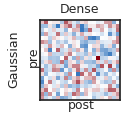
\includegraphics[width=\textwidth]{figures/ch3/Dense-Gaussian.png}
  \end{subfigure}
  ~
  \hspace{-.1in}
  \begin{subfigure}[b]{1.10in}
    \centering
    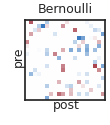
\includegraphics[width=\textwidth]{figures/ch3/Bernoulli-Gaussian.png}
  \end{subfigure}
  ~
  \hspace{-.1in}
  \begin{subfigure}[b]{1.10in}
    \centering
    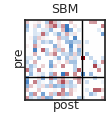
\includegraphics[width=\textwidth]{figures/ch3/SBM-Gaussian.png}
  \end{subfigure}
  ~
  \hspace{-.1in}
  \begin{subfigure}[b]{1.10in}
    \centering
    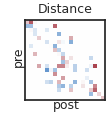
\includegraphics[width=\textwidth]{figures/ch3/Distance-Gaussian.png}
  \end{subfigure}
  \\
  \vspace{-.1in}
  % SBM row
  \rotatebox{90}{\textit{~~~~~Weight Model}}
  \begin{subfigure}[b]{1.25in}
    \centering
    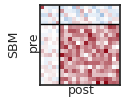
\includegraphics[width=\textwidth]{figures/ch3/Dense-SBM.png}
  \end{subfigure}
  ~
  \hspace{-.1in}
  \begin{subfigure}[b]{1.10in}
    \centering
    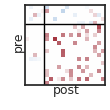
\includegraphics[width=\textwidth]{figures/ch3/Bernoulli-SBM.png}
  \end{subfigure}
  ~
  \hspace{-.1in}
  \begin{subfigure}[b]{1.10in}
    \centering
    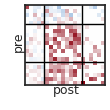
\includegraphics[width=\textwidth]{figures/ch3/SBM-SBM.png}
  \end{subfigure}
  ~
  \hspace{-.1in}
  \begin{subfigure}[b]{1.10in}
    \centering
    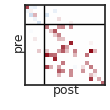
\includegraphics[width=\textwidth]{figures/ch3/Distance-SBM.png}
  \end{subfigure}
  \\
  % Distance row
  \vspace{-.1in}
  \hspace{1em}
  \begin{subfigure}[b]{1.25in}
    \centering
    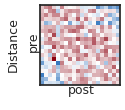
\includegraphics[width=\textwidth]{figures/ch3/Dense-Distance.png}
  \end{subfigure}
  ~
  \hspace{-.1in}
  \begin{subfigure}[b]{1.10in}
    \centering
    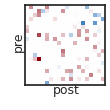
\includegraphics[width=\textwidth]{figures/ch3/Bernoulli-Distance.png}
  \end{subfigure}
  ~
  \hspace{-.1in}
  \begin{subfigure}[b]{1.10in}
    \centering
    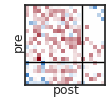
\includegraphics[width=\textwidth]{figures/ch3/SBM-Distance.png}
  \end{subfigure}
  ~
  \hspace{-.1in}
  \begin{subfigure}[b]{1.10in}
    \centering
    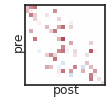
\includegraphics[width=\textwidth]{figures/ch3/Distance-Distance.png}
  \end{subfigure}
  \\
  \vspace{-.1in}
  \caption[Examples of network models]{Example network models.  Each
    row corresponds to a fixed weight matrix,~$\bW$, for three
    different weight models, and each column corresponds to a fixed
    adjacency matrix,~$\bA$, for four different adjacency models. The
    panels show the elementwise product of the two. Color denotes the
    weight (blue is negative, red is postiive).  In the SBM, the rows
    and columns are sorted by type, and in the distance model, they
    are sorted by location. }
  \label{fig:network_models}
\end{figure}

Figure~\ref{fig:network_models} shows how a variety of networks can be
constructed by combining different priors on the weights (rows) with
priors on the pattern of connectivity (columns). Each row corresponds
to a fixed weight matrix drawn from either an independent model, a
stochastic block model (SBM), or a latent distance model. In these
cases, the weights are Gaussian distributed with unit variance and
model-specific mean. Each column corresponds to a fixed adjacency
matrix drawn from either a dense model, an independent
Bernoulli model, an SBM, or a latent distance model. The matrices show
the element-wise product, which encodes a weighted, directed
network. 


\section{Hawkes Processes}
Hawkes processes \cite{Hawkes-1971} are a special type of point process
that allow spikes to influence the future firing rate. This is achieved
via a linear superposition of Poisson processes. Before jumping into the
details, a brief primer on point processes and Poisson processes is in
order.

\subsection{Poisson Processes}
\sloppy Point processes are fundamental statistical objects that yield
random finite sets of events~${\{s_m\}_{m=1}^M \subset \mcV}$,
where~$\mcV$ is a compact subset of~${\reals^D}$.  When modeling
neural spike trains, we typically let~${\mcV}$ equal the
interval~${[0,T]}$. The Poisson process is the canonical example. It
is governed by a nonnegative firing rate or intensity
function,~${\lambda(t): \mcV \rightarrow\reals_+}$. The number of
events in a subset~${\mcV'\subset\mcV}$ follows a Poisson distribution
with mean~${\int_{\mcV'}\lambda(t)\mathrm{d}t}$. Moreover, the number
of events in disjoint subsets are independent.

We use the notation~${\{s_m\}_{m=1}^M\sim\PP(\lambda(t))}$ to indicate
that a set of events~$\{s_m\}_{m=1}^M$ is drawn from a Poisson process
with rate~$\lambda(t)$. There are many ways to sample a Poisson
process; one way is to first sample a Poisson number of events with
mean~${\int_{\mcV} \lambda(t) \mathrm{d}t}$ and then sample the individual
event times,~$s_m$, independently from the density,
\begin{align*}
  p(t) &= \frac{\lambda(t)}{\int_{\mcV} \lambda(t) \, \mathrm{d}t}.
\end{align*}
Thus, after accounting for the~$M!$ permutations,
the likelihood of a set of events is given by,
\begin{align}
  \nonumber
  p(\{s_m\}_{m=1}^M \given \lambda(t))
  &= \distPoisson \left(M \, \bigg| \, \int_{\mcV} \lambda(t) \, \mathrm{d} t \right)
  \left( \prod_{m=1}^M \frac{\lambda(s_m)}{\int_{\mcV} \lambda(t) \, \mathrm{d}t} \right)  M! \\
  \nonumber
  &= \frac{M!}{M!} \left(\int_{\mcV} \lambda(t) \, \mathrm{d} t \right)^M
  \exp \left \{-\int_{\mcV} \lambda(t) \, \mathrm{d} t \right \} 
  \left( \prod_{m=1}^M \frac{\lambda(s_m)}{\int_{\mcV} \lambda(t) \, \mathrm{d}t} \right) \\
  \label{eq:poisson_lkhd}
  &=\exp\left\{-\int_{\mathcal{V}}\lambda(t)\mathrm{d}t \right\}
  \prod_{m=1}^M\lambda(s_m).
\end{align}


We will make use of a special property of Poisson processes, the
\emph{Poisson superposition principle}, which states that if
\begin{align*}
  \{s_{m}\}_{m=1}^{M} &\sim \PP(\lambda(t))\\
  \{s'_{m}\}_{m=1}^{M'} &\sim \PP(\lambda'(t))
\end{align*}
are independent Poisson process realizations, then
\begin{align*}
\{s_{m}\}_{m=1}^{M} \cup \{s'_{m}\}_{m=1}^{M'} \sim \PP(\lambda(t)+\lambda'(t)).
\end{align*}
Furthermore,~${\{s_m\}\sim\PP(\lambda(t)+\lambda'(t))}$ can be
\emph{thinned} into two independent Poisson processes by randomly and
independently assigning each event $s_m$ to the first process with
probability~$\frac{\lambda(s_m)}{\lambda(s_m)+\lambda'(s_m)}$ and to
second process otherwise. These results extend to the superposition of
multiple processes by induction.

\subsection{Including Spike History with Hawkes Processes}
Though Poisson processes have many nice properties, they cannot
capture interactions between events. For this we turn to a more
general model known as Hawkes processes \cite{Hawkes-1971}. A Hawkes
process consists of~$N$ point processes and gives rise to sets of
\emph{marked} events $\{s_m,c_m\}_{m=1}^M$,
where~${c_m\in\{1,\ldots,N\}}$ specifies the process on which
the~$m$-th event occurred.  Each of the~$N$ processes is a
\emph{conditionally Poisson process} with a rate~${\lambda_n(t\given
  \mcH_t)}$ that depends on the preceding
events,~$\mcH_t=\{s_n:s_n<t\}$.
%Each of the~$K$ processes is a \emph{conditionally Poisson process} with a rate~$\lambda_k(t\given H(t))$ that depends on the history of events up to time~$t$, denoted~${H(t)=\{s_n:s_n<t\}}$.
This allows for event-driven dynamics that are not possible in Poisson
processes.  Moreover, the Hawkes process reduces to a set of
independent Poisson processes when the firing rate is independent of
the history.

Hawkes processes have additive interactions. Each process has a
``background rate'' $\lambda_{0,n}(t)$, and each event~$s_m$ on
process ${c_m=n}$ adds a nonnegative impulse response~$h_{n \to
  n'}(t-s_m)$ to the intensity of other processes~$n'$. Causality and
locality of influence are enforced by requiring~$h_{n \to n'}(\Delta
t)$ to be zero for~${\Delta t \notin[0,\Delta t_{\mathsf{max}}]}$.

\begin{figure}[t]
\centering%
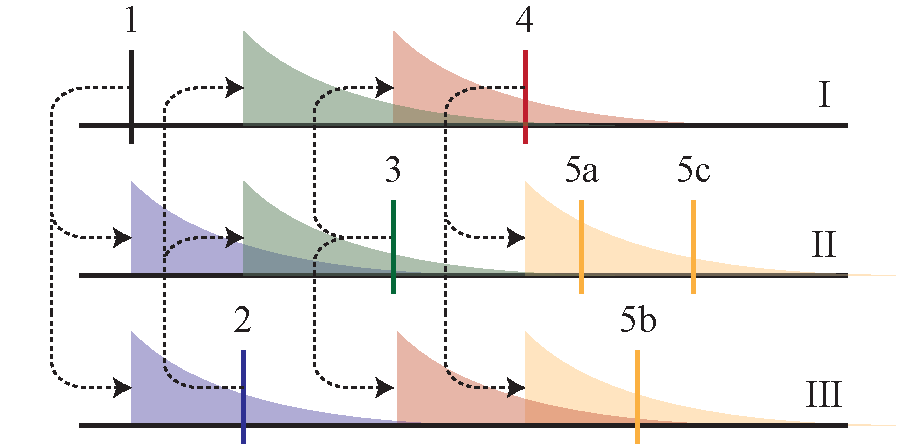
\includegraphics[width=\linewidth]{figures/ch2/Hawkes-wide} 
\vspace{-0.25cm}
\caption[Illustration of a Hawkes process]{Illustration of a Hawkes
  process. Events induce impulse responses on connected processes and
  spawn ``child'' events. See the main text for a complete
  description.}
\label{fig:hawkes}
\end{figure}

By the superposition theorem for Poisson processes, these additive
components can be considered independent processes, each giving rise
to their own events.  This suggests a convenient latent variable
representation in which each event is attributed to either the
background rate or the impulse response of a preceding event.  We
augment our data with a latent random
variable~${\omega_m \in\{0,\ldots, m-1\}}$ to indicate the \emph{origin} of
the~$n$-th event ($0$ if the event is due to the background rate and
${1\ldots m-1}$ if it was spawned by a preceding event). The augmented
Hawkes likelihood is then the product of likelihoods of each Poisson
process:
\begin{multline*}
p(\{(s_m,c_m,\omega_m)\}_{m=1}^M \given \{\lambda_{0,n}(t)\}, \{\{h_{n \to n'}(\Delta t)\}\}) = \\
\prod_{n=1}^N p(\{s_{m}: c_{m}=k \wedge \omega_{m}=0\} \given \lambda_{0,n}(t))\;\times\\
\prod_{m=1}^M \prod_{n=1}^N p(\{s_{m'}: c_{m'}=k \wedge \omega_{m'}=m\} \given h_{c_m \to n}(t-s_n)),
\end{multline*}
where the densities in the product are Poisson process likelihoods
given by Equation~\ref{eq:poisson_lkhd}.

Figure~\ref{fig:hawkes} illustrates a causal cascades of events for a
simple network of three processes (I-III).  The first event is caused
by the background rate~(${\omega_1=0}$), and it induces impulse responses
on processes II and III. Event~2 is spawned by the impulse on the
third process~(${\omega_2=1}$), and feeds back onto processes I and II. In
some cases a single parent event induces multiple children, e.g.,
event~4 spawns events~{5a-c}. In this simple example, processes excite
one another, but do not excite themselves. Next we will introduce more
sophisticated models for such interaction networks.

\section{The Network Hawkes Model}\label{sec:basic_model}
In order to combine Hawkes processes and random network models, we
decompose the Hawkes impulse response $h_{n \to n'}(\Delta t)$ as
follows:
\begin{align}
\label{eq:ir_decomp}
h_{n \to n'}(\Delta t) &= a_{n \to n'} \cdot w_{n \to n'} \cdot \hbar(\Delta t; \theta_{n \to n'}).
\end{align}
Here,~$a_{n \to n'}$ is an entry in the binary adjacency
matrix,~${\bA\in\{0,1\}^{N \times N}}$,
and~$w_{n \to n'}$ is the corresponding entry in the non-negative
weight matrix,~${\bW \in\reals_+^{N\times N}}$. Together these specify
the \emph{sparsity structure} and \emph{strength} of the interaction
network, respectively. The non-negative function~${\hbar(\Delta t;
  \theta_{n \to n'})}$ captures the temporal aspect of the
interaction. It is parameterized by~${\theta_{n \to n'}}$ and
satisfies two properties: a) it has bounded support for~${\Delta t \in
  [0,\Delta t_{\mathsf{max}}]}$, and~b) it integrates to one. In other
words,~$\hbar$ is a probability density with compact support.

Decomposing the impulse response as in Equation~\ref{eq:ir_decomp} has
many advantages. It allows us to express our separate beliefs about
the sparsity structure of the interaction network and the strength of
the interactions by using probabilistic network models as priors
on~$\bA$ and~$\bW$.  The empty graph model recovers independent
background processes, and the complete graph recovers the standard
Hawkes process introduced by \citet{Hawkes-1971}.  Making~$\hbar$ a
probability density endows~$\bW$ with units of ``expected number of
events'' and allows us to compare the relative strength of
interactions. The form suggests an intuitive generative model: for
each impulse response draw~${k \sim \text{Poisson}(w_{n \to n'})}$
number of induced events and draw the~$k$ child event times
i.i.d.\ from~$\hbar$. As we will see, this enables computationally
tractable conjugate priors.

Intuitively, the background rates,~$\lambda_{0,n}(t)$, explain events
that cannot be attributed to preceding events. In the simplest case
the background rate is constant. However, there are often fluctuations
in overall intensity that are shared among the processes, and not
reflective of process-to-process interaction, as we will see in the
daily variations in trading volume on the S\&P100 and the seasonal
trends in homicide. To capture these shared background fluctuations,
we use a sparse log Gaussian Cox process \cite{Moller-1998} to model
the background rate:
\begin{align*}
  \lambda_{0,n}(t)
  & = \mu_{n} + \alpha_{n}\exp\{\by(t)\}, \\
  \by(t) &\sim \mathcal{GP}(\boldsymbol{0},K(t,t')).
\end{align*}

The kernel~${K(t,t')}$ describes the covariance structure of the
background rate that is shared by all processes. For example, a
periodic kernel may capture seasonal or daily fluctuations. The
offset~${\mu_n}$ accounts for varying background intensities among
processes, and the scaling factor~$\alpha_n$ governs how sensitive
process~$n$ is to these background fluctuations (when~${\alpha_n=0}$
we recover the constant background rate).

Finally, in some cases the process identities,~${c_m}$, must also be
inferred. With gang incidents in Chicago we may have only a
location,~${\bx_m\in\reals^2}$. In this case, we may place a spatial
Gaussian mixture model over the~$c_m$'s, as in
\citet{Cho-2013}. Alternatively, we may be given the label of the
community in which the incident occurred, but we suspect that
interactions occur between clusters of communities. In this case we
can use a simple clustering model or a nonparametric model like that
of \citet{Blundell-2012}.

\subsection{Inference with Gibbs Sampling}
We present a Gibbs sampling procedure for inferring the model
parameters,~$\bA$,~$\bW$,~$\btheta$,$\{\lambda_{0,n}(t)\}$, and, if
necessary,~${\{c_m\}}$. In order to simplify our Gibbs updates, we
will also sample a set of parent assignments for each
event~$\{\omega_m\}$. Incorporating these parent variables enables
conjugate prior distributions for~$\bW$,~$\theta_{n \to n'}$, and, in
the case of constant background rates,~$\lambda_{0,n}$.

By combining
Equations~\ref{eq:poisson_lkhd}~and~\ref{eq:hawkes_likelihood}, we can
write the joint likelihood, with the auxiliary parent variables, as,
\begin{multline}
  \label{eq:complete_likelihood}
  p(\{s_m, c_m, \omega_m\}_{m=1}^M \given \{\lambda_{0,n}(t)\}_{n=1}^N, \{h_{n \to n'}(\Delta t)\}) = \\
  \prod^N_{n=1} \bigg[
  \exp\left\{ -\int_0^T \lambda_{0,n}(t)\mathrm{d}t \right\} \,
  \prod^M_{m=1}
   \lambda_{0,n}(s_m)^{\bbI[c_m=n] \bbI[\omega_m = 0]} \bigg]\\
  \quad\times \prod_{m=1}^M \prod_{n'=1}^N \bigg[
  \exp\left\{-\int^T_{s_m} h_{c_m,n'}(t - s_m) \mathrm{d}t \right\} \\
  \prod_{m'=1}^M h_{c_m^{~},c_{m'}}(s_{m'}-s_m)^{\bbI[c_{m'}=n'] \bbI[\omega_{m'}=m]}\bigg].
\end{multline}
The second line corresponds to the likelihood of the background
processes; the third and fourth correspond to the likelihood of the
induced processes triggered by each spike.

\paragraph{Sampling weights $\bW$.} 
To derive the updates for weights, recall from
Equation~\ref{eq:ir_decomp} that~${w_{n \to n'}}$ only
appears in the impulse responses for which~${c_m=n}$
and~${c_{m'}=n'}$, so the likelihood is propotional to,
\begin{align*}
  p(\{s_m,c_m, &\omega_m\}^M_{m=1} \given a_{n \to n'}, w_{n \to n'}, 
  \theta_{n \to n'}) \\
  &\propto \prod_{m=1}^M\left[
    \exp\left\{-\int^T_{s_m} a_{n \to n'} \cdot w_{n \to n'} \cdot \hbar(t - s_m; \theta_{n \to n'}) \, \mathrm{d}t
    \right\} \right]^{\bbI[c_m=n]} \\
  &\qquad \times \prod_{m=1}^M \prod_{m'=1}^M \bigg[
    w_{n \to n'}\bigg]^{\bbI[c_{m}=n] \bbI[c_{m'}=n'] \bbI[\omega_{m'}=m]}.
\end{align*}
If~${a_{n \to n'}=0}$, the impulse response is deterministically zero
and, as a result, no spikes on neuron~$n'$ will be attributed to spikes
on neuron~$n$. Thus, the likelihood reduces to the prior,~$p(w_{n \to n'})$.
If~${a_{n \to n'}=1}$, we have to consider the likelihood.
Assume that there are no spikes after~${T-\Delta t_{\mathsf{max}}}$. Then,
\begin{align*}
  -\int^T_{s_m} w_{n \to n'} \cdot
  \hbar(t - s_m; \theta_{n \to n'}) \, \mathrm{d}t
  &= -w_{n \to n'}  \int^T_{s_m} \hbar(t - s_m; \theta_{n \to n'}) \, \mathrm{d}t \\
  &= - w_{n \to n'},
\end{align*}
since~$\hbar$ is a density defined on~$[0,\Delta t_{\mathsf{max}}]$.
With this approximation, the conditional distribution of~$w_{n \to n'}$
reduces to,
\begin{align*}
  p(\{s_m,c_m, \omega_m\}^M_{m=1} \given a_{n \to n'}=1, w_{n \to n'}) 
  \propto 
  e^{-M_n \cdot w_{n \to n'}}  \,
  (w_{n \to n'})^{M_{n \to n'}}.
\end{align*}
where
\begin{align*}
  M_{n} &= \sum_{m=1}^M \bbI[c_{m}=n], \\
  M_{n \to n'} &= \sum_{m=1}^M \bbI[c_{m}=n] \, \bbI[c_{m'}=n'] \, \bbI[\omega_{m'}=m].
\end{align*}
These sufficient statistics correspond to the number of events caused
by an connection~${n \to n'}$ and the total unweighted rate induced by
events on neuron~$n$.

Now that we have simplified the augmented log likelihood, we see that it is
conjugate with a gamma prior on the weights,
${w_{n \to n'}\sim \distGamma(\alpha_w, \beta_w})$.
The resulting conditional distribution is,
\begin{multline*}
  p(w_{n \to n'}\given \{s_m,c_m,\omega_m\}_{m=1}^M, a_{n\to n'}=1, \alpha_w, \beta_w)
  = 
  \distGamma(w_{n \to n'} \given \widetilde{\alpha}_{n \to n'}, \widetilde{\beta}_{n \to n'}),
\end{multline*}
where
\begin{align*}
  \widetilde{\alpha}_{n \to n'} &= \alpha_w + M_{n \to n'}, \\
  \widetilde{\beta}_{n \to n'} &= \beta_w + M_n.
\end{align*}


\paragraph{Sampling constant background rates.}
Similarly, the likelihood of a constant background rate,
${\lambda_{0,n}(t)\equiv\lambda_{0,n}}$, is conjugate with a gamma
prior ${\lambda_{0,n} \sim
  \distGamma(\alpha_{\lambda},\beta_{\lambda})}$.  The conditional
distribution is,
\begin{align*}
  p(\lambda_{0,n} \given \{s_m,c_m, \omega_m\}_{m=1}^M, \alpha_\lambda, \beta_\lambda)
  &=
  \distGamma(\lambda_{0,n} \given \widetilde{\alpha}_{0,n},  \widetilde{\beta}_{0,n}),\\
  \widetilde{\alpha}_{0,n} &= \alpha_{\lambda} + \sum_m \bbI[c_m = n] \, \bbI[\omega_m=0] \\
  \widetilde{\beta}_{0,n} &= \beta_\lambda + T
\end{align*}

This conjugacy no longer holds for log Gaussian Cox process background
rates, but conditioned upon the parent variables, we must simply fit a
log Gaussian Cox process for those events for which~${\omega_m=0}$. We use
elliptical slice sampling \cite{Murray-2010} for this purpose.

\paragraph{Sampling impulse response parameters $\theta_{n \to n'}$.}
The logistic-normal density with parameters~${\theta_{n \to
    n'}=\{\mu_{n \to n'},\tau_{n \to n'}\}}$ provides a flexible model
for the impulse response:
\begin{align*}
  \hbar(\Delta t ; \,  \mu_{n \to n'}, \tau_{n \to n'})
  &=\frac{1}{Z}\exp\left\{\frac{-\tau_{n \to n'}}{2}
  \left(\sigma^{-1}\left(\frac{\Delta t}{\Delta t_{\mathsf{max}}}\right)
  - \mu_{n \to n'} \right)^2 \right\} \\
  \sigma^{-1}(x) &= \ln(x/(1-x))\\ Z &=
  \frac{\Delta t(\Delta t_{\sf{max}}-\Delta t)}{\Delta t_{\mathsf{max}}}
  \left(\frac{\tau_{n \to n'}}{2\pi}\right)^{-\frac{1}{2}}.
\end{align*}
Given the auxiliary parent variables, the likelihood is conjugate with
a normal-gamma prior~${\mu_{n \to n'},\tau_{n \to n'} \sim
  \mathcal{NG}(\mu_\mu,\kappa_\mu,\alpha_\tau,\beta_\tau)}$.
The sufficient statistics are,
\begin{align*}
x_{m \to m'} &\triangleq \ln(s_{m'}-s_m)-\ln(t_{\sf{max}}-(s_{m'}-s_m)), \\
%r_{n \to n'} &= \sum_{m=1}^M \sum_{m'=1}^M \bbI[c_m=n] \, \bbI[c_{m'}=n'] \, \bbI[\omega_{m'}=m], \\
\bar{x}_{n \to n'} &= \frac{1}{M_{n \to n'}} \sum_{m=1}^M \sum_{m'=1}^M \bbI[c_m=n] \, \bbI[c_{m'}=n'] \, \bbI[\omega_{m'}=m] \,x_{m \to m'}, \\
v_{n \to n'} &= \sum_{m=1}^M \sum_{m'=1}^M \bbI[c_m=n] \, \bbI[c_{m'}=n'] \, \bbI[\omega_{m'}=m] \, (x_{m \to m'} - \bar{x})^2.
\end{align*}
Intuitively, these correspond to the number of events caused by an
interaction and the mean and variance of their (transformed) delays.
%The conditional distribution is,
%\begin{align*}
%  \mu_{n \to n'},\tau_{n \to n'} \given \{s_m,c_m, \omega_m\}_{m=1}^M) &\sim
%  \mathcal{NG}(\mu_\mu,\kappa_\mu,\alpha_\tau,\beta_\tau)
%\end{align*}
The parameters of the normal-gamma conditional distribution are,
\begin{align*}
  \widetilde{\mu}_{n \to n'} &= \frac{\kappa_\mu \mu_\mu + M_{n \to n'} \bar{x}_{n \to n'}}{\kappa_\mu + M_{n \to n'}}, 
  &
  \widetilde{\kappa}_{n \to n'} &= \kappa_\mu + M_{n \to n'}, \\
  \widetilde{\alpha}_{n \to n'} &= \alpha_{\tau} + \frac{M_{n \to n'}}{2},
  & 
  \widetilde{\beta}_{n \to n'} &= \frac{v_{n \to n'}}{2} + \frac{M_{n \to n'} \kappa_\mu}{M_{n \to n'} + \kappa_\mu}\frac{(\bar{x}_{n \to n'} - \mu_\mu)^2}{2}.
\end{align*}

\paragraph{Collapsed Gibbs sampling $\bA$ and $\bomega$.}
With Aldous-Hoover graph priors, the entries in the binary adjacency
matrix~$\bA$ are conditionally independent given the parameters of the
prior. The likelihood introduces dependencies between the rows
of~$\bA$, but each column can be sampled in parallel. Gibbs updates
are complicated by strong dependencies between the graph and the
parent variables,~$\omega_m$. Specifically, if~${\omega_{m'}=m}$, then
we must have~${a_{c_{m},c_{m'}}=1}$. To improve the mixing of our
sampling algorithm, first we
update~${\bA\given\{s_m,c_m\},\bW,\theta_{n \to n'}}$ by marginalizing
the parent variables. The posterior is determined by the likelihood of
the conditionally Poisson process~${\lambda_{n'}(t\given \mcH_t)}$
(Eq.~\ref{eq:poisson_lkhd}) with and without interaction~${a_{n
    \to n'}}$ and the prior comes from the Aldous-Hoover graph
model. Then we update~${\omega_m \given \{s_m,c_m\},\bA,\bW,\theta_{n
    \to n'}}$ by sampling from the discrete conditional
distribution. Though there are~$M$ parent variables, they are
conditionally independent and may be sampled in parallel. We have
implemented our inference algorithm on GPUs to capitalize on this
parallelism.

\paragraph{Sampling process identities $c_m$.}
As with the adjacency matrix, we use a collapsed Gibbs sampler to
marginalize out the parent variables when sampling the process
identities. Unfortunately, the~$c_m$'s are not conditionally
independent and hence must be sampled sequentially.

\paragraph{Computational concerns.}
Compact impulse responses limit the number of potential event parents
and significantly reduce the memory requirements and running time of
our algorithm. If the average firing rate is constant, the expected
number of potential parents per event will be linear in $N$. Summing
the per-event contributions to the log likelihood can be done
in~${\mathrm{O}(\log M)}$ time using standard parallel
reductions. Hence, after parallelizing over the columns of $\bA$ and
the parents~$\omega_m$, one step of our sampling algorithm
takes~${\mathrm{O}(N(N+\log M))}$ time when process identities are
known, and~${\mathrm{O}((N+M)(N+\log M))}$ time otherwise. On the
datasets used in the following experiments, our GPU
implementation
%\footnote{\url{https://github.com/slinderman}}
achieves
5-50 iterations per second.

\section{Stability of Network Hawkes Processes}
\label{sec:stability}

\begin{figure*}[!ht]
\vspace{-.5em}
\begin{center}
\begin{subfigure}[b]{.22\textwidth}
\caption{}
\label{fig:stability_p_w}
%\vspace{-.9em}
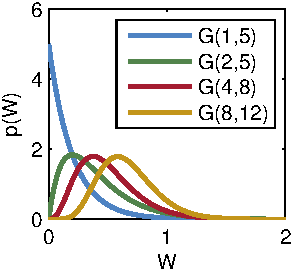
\includegraphics[height=1.35in]{figures/ch2/stability_p_w} 
\end{subfigure}
~
\begin{subfigure}[b]{.22\textwidth}
\caption{}
%\vspace{-1em}
\label{fig:stability_max_rho}
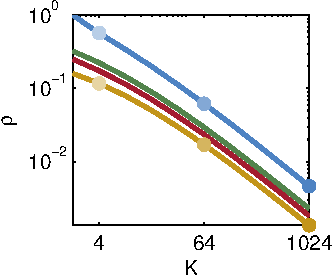
\includegraphics[height=1.35in]{figures/ch2/stability_max_rho} 
\end{subfigure}
~
\hspace{1em}
\begin{subfigure}[b]{.22\textwidth}
\caption{}
\label{fig:stability_1_5}
%\vspace{-.5em}
%\vspace{.8em}
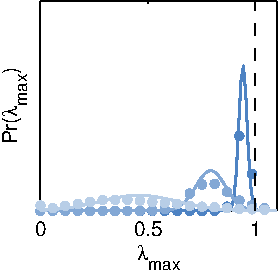
\includegraphics[height=1.3in]{figures/ch2/stability_1_5} 
\end{subfigure}
~
\begin{subfigure}[b]{.22\textwidth}
%\vspace{.7em}
\caption{}
\label{fig:stability_8_12}
%\vspace{-.5em}
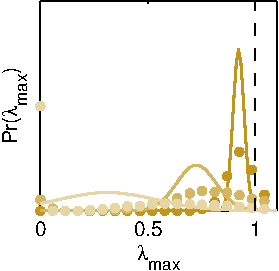
\includegraphics[height=1.3in]{figures/ch2/stability_8_12} 
\end{subfigure}
\end{center}
\vspace{-1em}
\caption[Distribution of the maximum eigenvalue for Erd\H{o}s-Renyi
  graphs with gamma weights]{Empirical and theoretical distribution of
  the maximum eigenvalue for Erd\H{o}s-Renyi graphs with gamma
  weights. (a) Four gamma weight distributions. The colors correspond
  to the curves in the remaining panels. (b) Sparsity that
  theoretically yields ${99\%}$ probability of stability as a function
  of~${p(W)}$ and~$N$. (c) and (d) Theoretical (solid) and empirical
  (dots) distribution of the maximum eigenvalue. Color corresponds to
  the weight distribution in (a) and intensity indicates~$N$
  and~$\rho$ shown in (b).}
\label{fig:stability}
\end{figure*}

Due to their recurrent nature, Hawkes processes must be constrained to
ensure their positive feedback does not lead to infinite numbers of
events. A stable system must satisfy
%\footnote{In this
%  context~${\lambda_{\mathsf{max}}}$ refers to an eigenvalue rather
%  than a rate, and~$\odot$ denotes the Hadamard product.}
\begin{align*}
  \lambda_{\mathsf{max}}=\max\; |\,\mathrm{eig}(\bA\odot\bW)\,| < 1
\end{align*}
(c.f. \citet{Daley-1988}). When we are conditioning on finite datasets
we do not have to worry about this. We simply place weak priors on the
network parameters, e.g., a beta prior on the sparsity~${\rho}$ of an
Erd\H{o}s-Renyi graph, and a Jeffreys prior on the scale of the gamma
weight distribution. For the generative model, however, we would like
to set our hyperparameters such that the prior distribution places
little mass on unstable networks. In order to do so, we use tools from
random matrix theory.

The circular law describes the asymptotic eigenvalue distribution for
$N \times N$~random matrices with entries that are i.i.d. with zero
mean and variance~$\sigma^2$. As~$N$ grows, the eigenvalues are
uniformly distributed over a disk in the complex plane centered at the
origin and with radius~$\sigma\sqrt{N}$. In our case, however, the
mean of the entries,~${\mu=\mathbb{E}[a_{n \to n'} \cdot w_{n \to
      n'}]}$, is not zero. \citet{Silverstein-1994} has analyzed such
``noncentral'' random matrices and shown that the largest eigenvalue
is asymptotically distributed
as~${\lambda_{\sf{max}} \sim \distNormal(\mu N,\, \sigma^2)}$.

% Replacing this paragraph with the simple statement that
%\lambda_{\sf{max}}\sim\distNormal(\mu K, \sigma^2).
%\citet{Silverstein-1994} has shown that we can analyze noncentral
%random matrices by considering them to be perturbations about the
%mean. Consider~${\bA\odot\bW=\bV+\bU}$, where~${\bV=\mu K e_K e_K^T}$
%is a deterministic rank-one matrix with every entry equal to~$\mu$,
%${e_K\in\reals^K}$ is a column vector with all entries equal
%to~${K^{-1/2}}$, and~$\bU$ is a random matrix with i.i.d.\ zero-mean
%entries. Then, as~$K$ approaches infinity, the largest eigenvalue
%will come from~$\bV$ and will be distributed
%as~${\lambda_{\sf{max}}\sim\distNormal(\mu K, \sigma^2)}$, and the
%remaining eigenvalues will be uniformly distributed over the complex
%disc.

In the simple case of~${w_{n \to n'}\sim \distGamma(\alpha,\beta)}$
and~${a_{n \to n'}\sim\distBernoulli(\rho)}$, we have ${\mu = \rho
  \alpha/\beta}$ and
${\sigma=\sqrt{\rho((1-\rho)\alpha^2+\alpha)}/\beta}$. For a
given~$N$,~$\alpha$ and~$\beta$, we can tune the sparsity
parameter~$\rho$ to achieve stability with high probability. We simply
set~$\rho$ such that the minimum of~$\sigma\sqrt{N}$ and, say,~${\mu N
  + 3\sigma}$, equals one. Figures~\ref{fig:stability_p_w}
and~\ref{fig:stability_max_rho} show a variety of weight distributions
and the maximum stable~$\rho$. Increasing the network size, the mean,
or the variance will require a concomitant increase in sparsity.

This approach relies on asymptotic eigenvalue distributions, and it is
unclear how quickly the spectra of random matrices will converge to
this distribution. To test this, we computed the empirical eigenvalue
distribution for random matrices of various size, mean, and
variance. We generated~$10^4$ random matrices for each weight
distribution in Figure~\ref{fig:stability_p_w} with sizes~$N=4$,~$64$,
and~$1024$, and~$\rho$ set to the theoretical maximum indicated by
dots in Figure~\ref{fig:stability_max_rho}. The theoretical and
empirical distributions of the maximum eigenvalue are shown in
Figures~\ref{fig:stability_1_5} and~\ref{fig:stability_8_12}. We find
that for small mean and variance weights, for
example~$\distGamma(1,5)$ in the Figure~\ref{fig:stability_1_5}, the
empirical results closely match the theory. As the weights grow
larger, as in~${\distGamma(8,12)}$ in~\ref{fig:stability_8_12}, the
empirical eigenvalue distributions have increased variance and lead to
a greater than expected probability of unstable matrices for the range
of network sizes tested here. We conclude that networks with strong
weights should be counterbalanced by strong sparsity limits, or
additional structure in the adjacency matrix that prohibits excitatory
feedback loops.

\section{Synthetic Results}
\label{sec:synth}
Our inference algorithm is first tested on synthetic data generated
from the network Hawkes model. We perform two tests: a) a link
prediction task where the process identities are given and the goal is
to simply infer whether or not an interaction exists, and b) an event
prediction task where we measure the probability of held-out event
sequences.

The network Hawkes model can be used for link prediction by
considering the posterior probability of interactions~$P(a_{n \to
  n'}\given \{s_m,c_m\})$. By thresholding at varying probabilities we
compute a ROC curve. A standard Hawkes process assumes a complete set
of interactions~($a_{n \to n'}\equiv 1$), but we can similarly threshold
its inferred weight matrix to perform link prediction.

Cross correlation provides a simple alternative measure of
interaction. By summing the cross-correlation over offsets~${\Delta
  t\in[0,\Delta t_{\mathsf{max}})}$, we get a measure of directed
  interaction. A probabilistic alternative is offered by the
  generalized linear model for point processes (GLM), a popular model
  for spiking dynamics in computational neuroscience
  \cite{Paninski-2004}. The GLM allows for constant background rates
  and both excitatory and inhibitory interactions. Impulse responses
  are modeled with linear basis functions. Area under the impulse
  response provides a measure of directed excitatory interaction that
  we use to compute a ROC curve. See the supplementary material for a
  detailed description of this model.
\begin{figure}[t]
  \begin{center}
  \begin{subfigure}[T]{.4\textwidth}
    \caption{}
    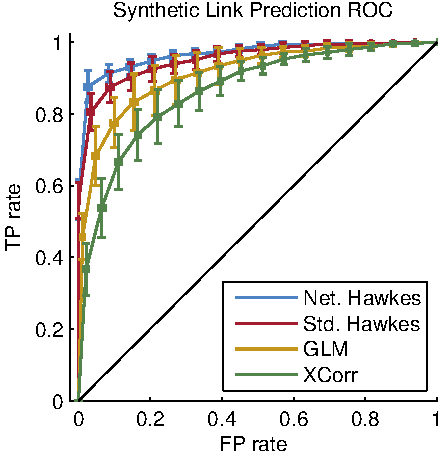
\includegraphics[width=\textwidth]{figures/ch2/synth_link_pred} 
    \label{fig:synth_link_pred}
  \end{subfigure}
  ~
  \begin{subfigure}[T]{.4\textwidth}
    \caption{}
    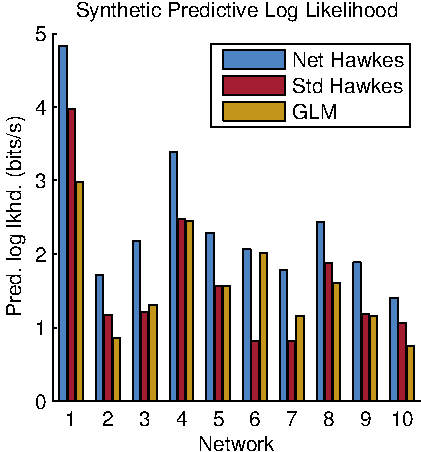
\includegraphics[width=\textwidth]{figures/ch2/synth_pred_ll}
    \label{fig:synth_pred_ll}
  \end{subfigure}
  \end{center}
  \vspace{-1em}
  \caption[Synthetic link prediction and predictive log likelihood]{
    \textbf{(a)} Comparison of models on a link prediction test
    averaged across ten randomly sampled synthetic networks of 30
    nodes each. The network Hawkes model with the correct
    Erd\H{o}s-Renyi graph prior outperforms a standard Hawkes model,
    GLM, and simple thresholding of the cross-correlation matrix.
    \textbf{(b)} Comparison of predictive log likelihoods, compared to
    a baseline of a Poisson process with constant rate. Improvement in
    predictive likelihood over baseline is normalized by the number of
    events in the test data to obtain units of ``bits per spike.'' The
    network Hawkes model outperforms the competitors in all sample
    networks.}
\end{figure}

% Table of results
\begin{table}
  \begin{center}
    \begin{tabular}{l|c}
      \textbf{Financial Model} & \textbf{Pred. log lkhd. (bits/spike)} \\
      \hline
      Indep. LGCP & $0.594$ \\
      Std. Hawkes & $0.912$ \\
      Net. Hawkes (Erd\H{o}s-Renyi) & $0.903$ \\
      Net. Hawkes (Latent Distance) & $0.888$ \\
      %Net. Hawkes (SBM) & $0.894$ \\
    \end{tabular}
  \end{center}
    \caption{Comparison of financial models on a event prediction task, relative to a homogeneous Poisson process baseline.}
    \label{tab:financial_pred_ll}
\end{table}

We sampled ten network Hawkes processes of~$30$ nodes each with
Erd\H{o}s-Renyi graph models, constant background rates, and the
priors described in Section~\ref{sec:basic_model}. The Hawkes
processes were simulated for~${T=1000}$ seconds. We used the models
above to predict the presence or absence of interactions. The results
of this experiment are shown in the ROC curves of
Figure~\ref{fig:synth_link_pred}. The network Hawkes model accurately
identifies the sparse interactions, outperforming all other models.
With the Hawkes process and the GLM we can evaluate the log likelihood
of held-out test data. On this task, the network Hawkes outperforms
the competitors for all networks. On average, the network Hawkes model
achieves~$2.2\pm.1$ bits/spike improvement in predictive log
likelihood over a homogeneous Poisson
process. Figure~\ref{fig:synth_pred_ll} shows that on average the
standard Hawkes and the GLM provide only 60\% and 72\%, respectively,
of this predictive power. See the supplementary material for further
analysis.

\begin{figure}[t]
  \vspace{-1em}
  \begin{center}
    \begin{subfigure}[T]{.75\textwidth}
      \centering
      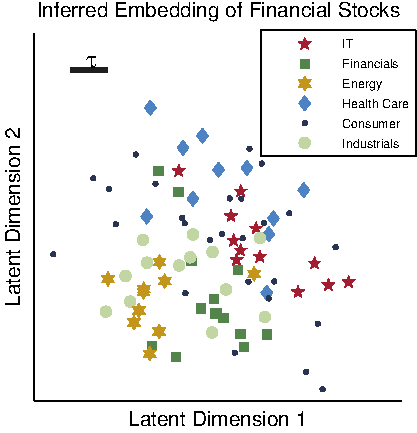
\includegraphics[width=.65\linewidth]{figures/ch2/financial_embedding} 
  \end{subfigure}
  \\
  \vskip1ex
  \begin{subfigure}[T]{.75\textwidth}
    \centering
    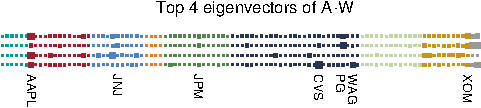
\includegraphics[width=\textwidth]{figures/ch2/financial_hinton} 
  \end{subfigure}
  \end{center}
  \vspace{-.5em}
  \caption[Financial embedding and dynamics eigenvectors]{
    \textbf{Top}: A sample from the posterior distribution over
    embeddings of stocks from the six largest sectors of the S\&P100
    under a latent distance graph model with two latent
    dimensions. Scale bar: the characteristic length scale of the
    latent distance model. The latent embedding tends to embed stocks
    such that they are nearby to, and hence more likely to interact
    with, others in their sector.
    \textbf{Bottom}: Hinton diagram of
    the top 4 eigenvectors. Size indicates magnitude of each stock's
    component in the eigenvector and colors denote sectors as in the
    top panel, with the addition of Materials (aqua), Utilities
    (orange), and Telecomm (gray). We show the eigenvectors
    corresponding to the four largest eigenvalues
    ${\lambda_{\mathsf{max}}=0.74}$ (top row) to ${\lambda_4=0.34}$
    (bottom row).}
  \label{fig:financial_embedding}
\end{figure}

\section{Trades on the S\&P 100}
\label{sec:financial}
As an example of how Hawkes processes may discover interpretable
latent structure in real-world data, we study the trades on the
S\&P~100 index collected at 1s intervals during the week of Sep.~28
through Oct.~2,~2009. Every time a stock price changes by~${\pm0.1\%}$
of its current price an event is logged on the stock's process,
yielding a total of~${N=100}$ processes and~${M=182,037}$ events.

Trading volume varies substantially over the course of the day, with
peaks at the opening and closing of the market. This daily variation
is incorporated into the background rate via a log Gaussian Cox
process (LGCP) with a periodic kernel (see supplementary material). We
look for short-term interactions on top of this background rate with
time scales of~${\Delta t_{\textsf{max}}=60\mathrm{s}}$.

% Chicago results
\begin{figure}[!t]
  \begin{center}
    \begin{subfigure}[T]{.32\textwidth}
      \begin{subfigure}[T]{\textwidth}
        \begin{center}
          \caption{}
          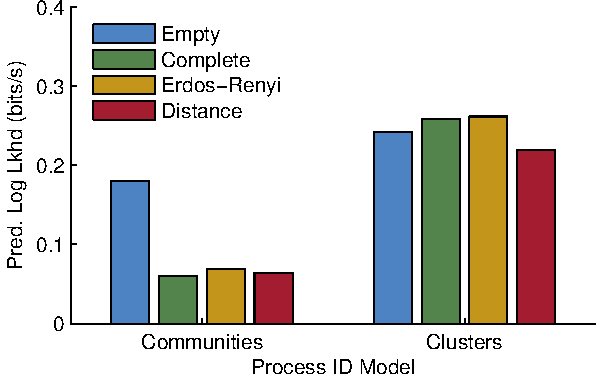
\includegraphics[width=\linewidth]{figures/ch2/icpsr_pred_ll}
          \label{fig:chicago_predll}
        \end{center}
      \end{subfigure}
      \begin{subfigure}[B]{\textwidth}
        \vspace{1em}
        \begin{center}
          \caption{}
          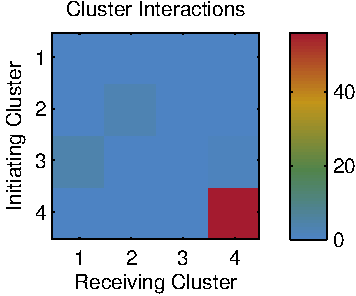
\includegraphics[width=.7\linewidth]{figures/ch2/icpsr_interactions}\\
          \label{fig:chicago_interactions}
        \end{center}
      \end{subfigure}
    \end{subfigure}
    ~
    \begin{subfigure}[B]{.32\textwidth}
      \caption{}
      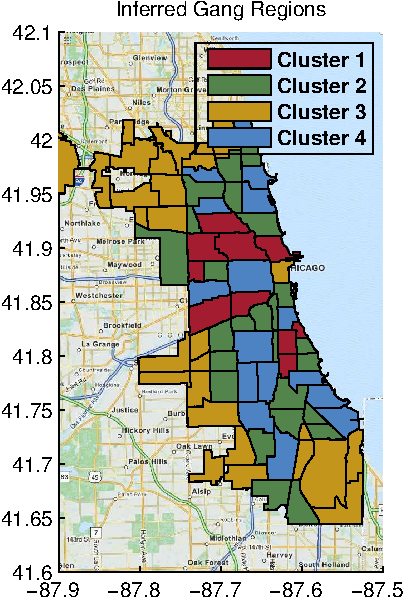
\includegraphics[width=\linewidth]{figures/ch2/icpsr_map} 
      \label{fig:chicago_map}
    \end{subfigure}
    \begin{subfigure}[B]{.28\textwidth}
      \caption{}
      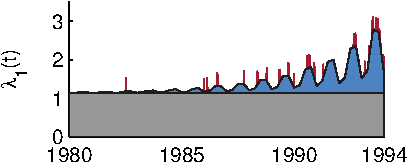
\includegraphics[width=\linewidth]{figures/ch2/icpsr_rate1} \\
      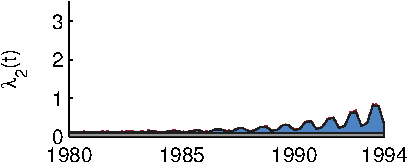
\includegraphics[width=\linewidth]{figures/ch2/icpsr_rate2} \\ 
      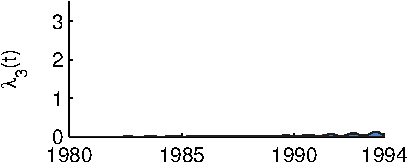
\includegraphics[width=\linewidth]{figures/ch2/icpsr_rate3} \\
      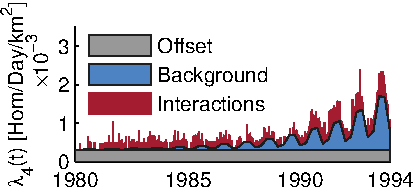
\includegraphics[width=\linewidth]{figures/ch2/icpsr_rate4} 
      \label{fig:chicago_rates}
    \end{subfigure}
  \end{center}
\vspace{-1em}
\caption[Inferred gang interactions in the city of Chicago]{
  Inferred interactions among clusters of community areas in the city of Chicago.
  \textbf{(a)} Predictive log likelihood for ``communities'' and ``clusters''  process identity models and four graph models. 
%Empty corresponds to independent LGCPs and Complete corresponds to the standard Hawkes process. 
  Panels \textbf{(b-d)} present results for the model with the highest predictive log likelihood: an Erd\H{o}s-Renyi graph with~${N=4}$ clusters.
  \textbf{(b)} The weighted interaction network in units of induced homicides over the training period (1980-1993).
  \textbf{(c)} Inferred clustering of the 77 community areas.
  \textbf{(d)} The intensity for each cluster, broken down into the offset, the shared background rate, and the interactions (units of~${10^{-3}}$ homicides per day per square kilometer).}
\label{fig:chicago}
\end{figure}

In Figure~\ref{tab:financial_pred_ll} we compare the
predictive performance of independent LGCPs, a standard Hawkes process
with LGCP background rates, and the network Hawkes model with LGCP
background rates under two graph priors. The models are trained on
four days of data and tested on the fifth. Though the network Hawkes
is slightly outperformed by the standard Hawkes, the difference is
small relative to the performance improvement from considering
interactions, and the inferred network parameters provide
interpretable insight into the market structure.

In the latent distance model for~$\bA$, each stock has a latent
embedding~${\bx_k\in\reals^2}$ such that nearby stocks are more likely
to interact, as described in
Section~\ref{sec:graph_models}. Figure~\ref{fig:financial_embedding}
shows a sample from the posterior distribution over embeddings
in~$\reals^2$ for~${\rho=0.2}$ and~${\tau=1}$. We have plotted stocks
in the six largest sectors, as listed on Bloomberg.com. Some sectors,
notably energy and financials, tend to cluster together, indicating an
increased probability of interaction between stocks in the same
sector. Other sectors, such as consumer goods, are broadly
distributed, suggesting that these stocks are less influenced by
others in their sector. For the consumer industry, which is driven by
slowly varying factors like inventory, this may not be surprising.

The Hinton diagram in the bottom panel of
Figure~\ref{fig:financial_embedding} shows the top 4 eigenvectors of
the interaction network. All eigenvalues are less than 1, indicating
that the system is stable. The top row corresponds to first
eigenvector~(${\lambda_{\mathsf{max}}=0.74}$). Apple~(\texttt{AAPL}),
J.P. Morgan~(\texttt{JPM}), and Exxon Mobil~(\texttt{XOM}) have
notably large entries in the eigenvector, suggesting that their
activity will spawn cascades of self-excitation.
% Removing this since it is entirely speculative
%The fourth eigenvector~(${\lambda_4=0.34}$) is dominated by Walgreens~(\texttt{WAG}) and CVS~(\texttt{CVS}), suggesting bursts of activity in these drug stores.
%, perhaps due to encouraging quarterly reports during flu season \cite{Walgreens-NYT-2009}.

\section{Gangs of Chicago}
\label{sec:chicago}
In our final example, we study spatiotemporal patterns of gang-related
homicide in Chicago. Sociologists have suggested that gang-related
homicide is mediated by underlying social networks and occurs in
mutually-exciting, retaliatory patterns \cite{Papachristos-2009}. This
is consistent with a spatiotemporal Hawkes process in which processes
correspond to gang territories and homicides incite further homicides
in rival territories.

We study gang-related homicides between 1980 and 1995
\cite{ICPSR}. Homicides are labeled by the community in which they
occurred. Over this time-frame there were~${M=1637}$ gang-related
homicides in the~${77}$ communities of Chicago.

We evaluate our model with an event-prediction task, training on
1980-1993 and testing on 1994-1995. We use a LGCP temporal background
rate in all model variations. Our baseline is a single process with a
uniform spatial rate for the city.  We test two process identity
models: a)~the ``community'' model, which considers each community a
separate process, and b)~the ``cluster'' model, which groups
communities into processes. The number of clusters is chosen by
cross-validation (see supplementary material). For each process
identity model, we compare four graph models: a)~independent LGCPs
(\emph{empty}), b)~a standard Hawkes process with all possible
interactions (\emph{complete}), c)~a network Hawkes model with a
sparsity-inducing Erd\H{o}s-Renyi graph prior, and d)~a network Hawkes
model with a latent distance model that prefers short-range
interactions.

The community process identity model improves predictive performance
by accounting for higher rates in South and West Chicago where gangs
are deeply entrenched. Allowing for interactions between community
areas, however, results in a decrease in predictive power due to
overfitting (there is insufficient data to fit all~${77^2}$ potential
interactions). Interestingly, sparse graph priors do not help. They
bias the model toward sparser but stronger interactions which are not
supported by the test data. These results are shown in the
``communities'' group of Figure~\ref{fig:chicago_predll}. Clustering
the communities improves predictive performance for all graph models,
as seen in the ``clusters'' group. Moreover, the clustered models
benefit from the inclusion of excitatory interactions, with the
highest predictive log likelihoods coming from a four-cluster
Erd\H{o}s-Renyi graph model with interactions shown in
Figure~\ref{fig:chicago_interactions}. Distance-dependent graph priors
do not improve predictive performance on this dataset, suggesting that
either interactions do not occur over short distances, or that local
rivalries are not substantial enough to be discovered in our
dataset. More data is necessary to conclusively say which.

Looking into the inferred clusters in Figure~\ref{fig:chicago_map} and
their rates in~\ref{fig:chicago_rates}, we can interpret the clusters
as ``safe suburbs'' in gold, ``buffer neighborhoods'' in green, and
``gang territories'' in red and blue. Self-excitation in the blue
cluster (Figure~\ref{fig:chicago_interactions}) suggests that these
regions are prone to bursts of activity, as one might expect during a
turf-war. This interpretation is supported by reports of ``a burst of
street-gang violence in 1990 and 1991'' in West Englewood
(${41.77^\circ}$N, ${-87.67^\circ}$W) \cite{Block-1993}.

Figure~\ref{fig:chicago_rates} also shows a significant increase in
the homicide rate between 1989 and 1995, consistent with reports of
escalating gang warfare \cite{Block-1993}. In addition to this
long-term trend, homicide rates show a pronounced seasonal effect,
peaking in the summer and tapering in the winter. A LGCP with a
quadratic kernel point-wise added to a periodic kernel captures both
effects.

\section{Related Work}
\citet{Gomez-2010} introduced one of the earliest algorithms for
discovering latent networks from cascades of events. They developed a
highly scalable approximate inference algorithm, but they did not
explore the potential of random network models or emphasize the point
process nature of the data.
%Coupling their approach with the random network models studied here
%could lead to scalable and insightful models.  Multivariate point
%processes are of great interest to the machine learning community as
%they are intuitive models for a variety of natural phenomena. We have
%leveraged previous work on Poisson processes with Gaussian process
%intensities in our background rate models \cite{Cunningham-2008}.
\citet{Simma-2010} studied this problem from the context of Hawkes
processes and developed an expectation-maximization inference
algorithm.
%An expectation-maximization inference algorithm for Hawkes processes
%was put forth by \citet{Simma-2010} and applied to very large social
%network datasets.
We have adapted their latent variable formulation in our
fully-Bayesian inference algorithm and introduced a framework for
prior distributions over the latent network.

Others have considered special cases of the model we have
proposed. \citet{Blundell-2012} combine Hawkes processes and the
Infinite Relational Model (a specific exchangeable graph model with an
Aldous-Hoover representation) to cluster processes and discover
interactions. \citet{Cho-2013} applied Hawkes processes to gang
incidents in Los Angeles. They developed a spatial Gaussian mixture
model (GMM) for process identities, but did not explore structured
network priors. We experimented with this process identity model but
found that it suffers in predictive log likelihood tests (see
supplementary material).

Recently, \citet{Iwata-2013} developed a stochastic EM algorithm for
Hawkes processes, leveraging similar conjugacy properties, but without
network priors. \citet{Zhou-2013} have developed a promising
optimization-based approach to discovering low-rank networks in Hawkes
processes, similar to some of the network models we explored.

\citet{Perry-2013} derived a partial likelihood inference algorithm
for Hawkes processes with a similar emphasis on structural patterns in
the network of interactions. They provide an estimator capable of
discovering homophily
%(the tendency for similar processes to interact) 
and other network effects. Our fully-Bayesian approach generalizes
this method to capitalize on recent developments in random network
models \cite{Lloyd-2012}.
% and allows for nonparametric background rates.

Finally, generalized linear models (GLMs) are widely used in
computational neuroscience \cite{Paninski-2004}. GLMs allow for both
excitatory and inhibitory interactions, but, as we have shown, when
the data consists of purely excitatory interactions, Hawkes processes
outperform GLMs in link- and event-prediction tests.

\section{Conclusion}\label{discussion}
%We developed a framework for discovering directed network structure
%in spiking datasets. We introduced an auxiliary variable formulation
%of the multivariate Hawkes process which supports arbitrary
%Aldous-Hoover graph priors, Gaussian process background rates, and
%models of unobserved process identities. Our Markov chain Monte Carlo
%algorithm leverages conjugate priors and several opportunities for
%parallelism. Additionally, we leveraged results from random matrix
%theory to analyze the conditions under which some random network
%models will be stable. Our applications uncovered interpretable
%latent networks in a variety of synthetic and real-world problems.

%Networks are powerful tools for describing the interactions we
%observe in nearly all areas of science. However, these networks are
%not always explicitly observable. Our fully-Bayesian approach allows
%us to reason about uncertainty in the latent network structure,
%taking into account noisy observations and prior beliefs. This work
%unites implicit network models and Hawkes process
%observations. Generalizing this framework to other observation models
%is a promising future direction.

We developed a framework for discovering latent network structure from
spiking data. Our auxiliary variable formulation of the multivariate
Hawkes process supported arbitrary Aldous-Hoover graph priors, log
Gaussian Cox process background rates, and models of unobserved
process identities.
%With parallel MCMC, we reasoned about uncertainty in the latent network in a fully-Bayesian manner. 
Our parallel MCMC algorithm allowed us to reason about uncertainty in
the latent network in a fully-Bayesian manner.  We leveraged results
from random matrix theory to analyze the conditions under which random
network models will be stable, and our applications uncovered
interpretable latent networks in a variety of synthetic and real-world
problems.
%Generalizing beyond the Hawkes observation model is a promising avenue for future work.


